\chapter{Interference}
\section{Interference}
Light wave is a harmonic electromagnetic wave consisiting of periodically varying electric and magnetic field oscillating at right angles to each other and also the direction of propagation of the wave.However the light wave is often represented by the  E wave since the many of the effect of light such as photoelectric effect ,photochemical physiological actions are found to be mostly due to the electric vector E.\\
\begin{figure}[H]
	\centering
	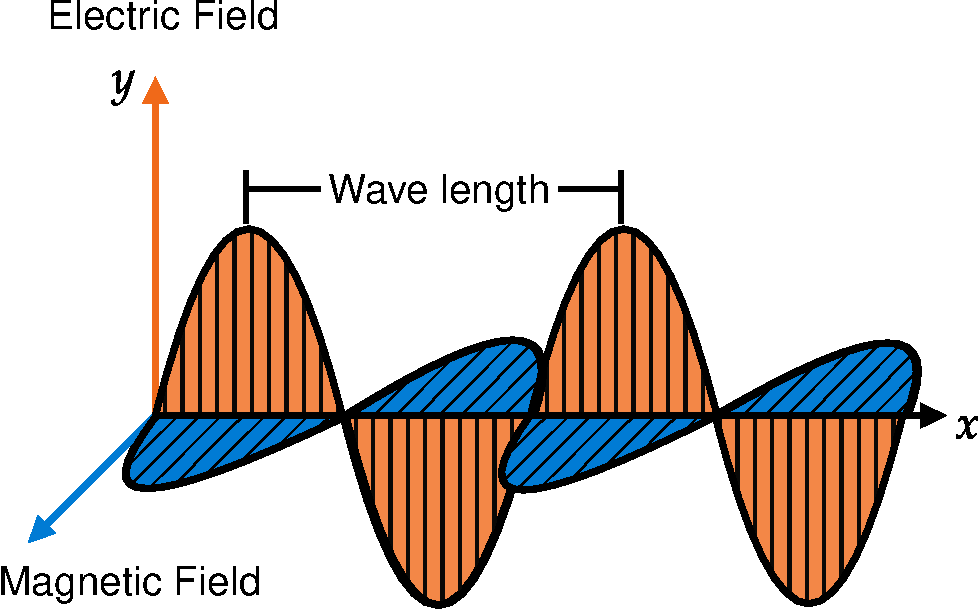
\includegraphics[height=3cm,width=5cm]{9.0-crop}
	\caption{}
	\label{}
\end{figure}
The light wave depicted in figure mathematically represented by the expression\\
$$E=E_{0}\sin (kz-\omega t)$$
\subsection{Some important points about light}
\begin{enumerate}
	\item characterestics of an ideal wave\\
	(a) The wave has a sigle definite frequency $\nu$ ($=\omega/2\pi$)\\
	The single frequency waves are called monochromatic waves\\
	(b)It is a harmonic wave and is of infinite extension consisiting of a continuous  train of waves.At any instant the wave extentd from $z=-\infty$ and $z=+\infty$\\
	(c) The amplitude of the wave $E_0$ stays constant as the wave propagates through the air.\\
	(d)The elcectric vector E of the wave oscillates always parallel to the fixed direction in space  ie y direction .Therefore the wave is plane polarized or linear polarized.
	\par The real light waves emitted by common light sources are far from real. They are wave trans of limited length, have a spread of frequencies, and are not plane polarized.  The common light sources emit a continuous distribution of wavelengths. The sodium lamp used in optics laboratories is a fairly monochromatic source of light, which emits light in the yellow region at the wavelength $5893 \AA$. The most nearly monochromatic source is the heliumneon laser that emits red light at $6328 \AA$.
	\item  A light wave travels slower in an optical medium than in air or a vacuum. It travels with a velocity $v$, which is less than ' $c$ '. The wavelength of light wave decreases in the medium, while its frequency remains constant.
	\item \textbf{Phase difference and coherence}\\
	\textbf{Coherent waves} If we consider two waves of same frequency ,they may differ in amplitude but they maintain a predictable phase relationship.The difference in their phases may have any value from zero radians to a maximum of 2$\pi$ radians;but the phase difference remains the constant.Thus two or more waves of the same frequency can maintain the same phase or constant phase difference over a distance and time  is called a coherent wave.\\
	\textbf{incoherent waves} If one or both of the waves undergoes change in frequency irregularly .Under these conditions thsese waves are said to be incoherent. The light emitted by most of the light sources is incoherent as the frequency of light changes abruptly and irregularly.\\
	\textbf{In phase}
	When coherent rise and fall together reaching crest at the same time they are said to be in phase.\\
	\textbf{Opposite phase} When one wave reaches its crests while the other falls to its trough,Then the phase difference betweeen the wave is $\pi$ and the wave is said to be opposite phase.
	\begin{figure}[H]
		\centering
		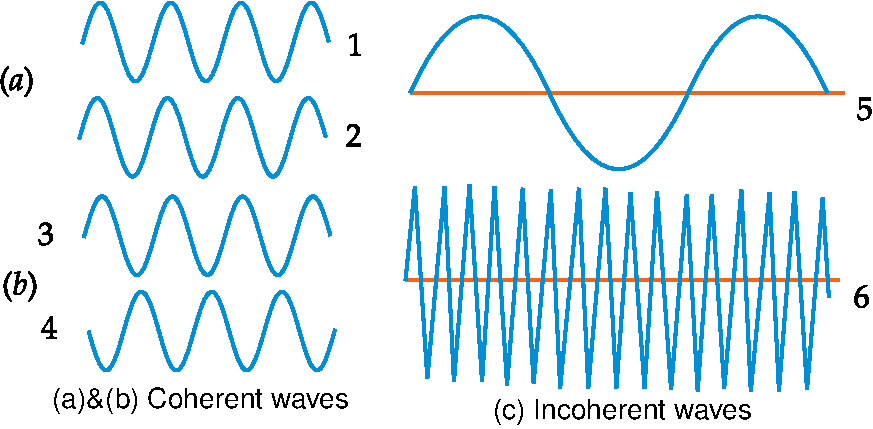
\includegraphics[height=5cm,width=10cm]{diagram-20211216(10)-crop}
		\caption{(a)Waves 1 and 2 are in phase(b)waves 3 and 4 are in opposite phase and (c)waves 5 and 6 are incoherent}
		\label{}
	\end{figure}
	\item \textbf{Optical path and phase change}\\
	Optical path is related to the geometric path and the relation may be found as follows. distance traversed by light in a medium of refractive index $\mu$ in time $t$ is given by
	$$
	L=v t
	$$
	are $v$ is the velocity of light in the medium.\\
	The distance travelled by light in a vacuum in the me time $t$, is $$\Delta=c t=c \cdot \frac{L}{v}=\mu L$$
	
	The distance $\mathrm{L}$ is called the geometric path length (GPL). $\Delta$ is the equivalent distance in vacuum and is called optical path length (OPL). Thus,
	$$
	\begin{aligned}
	\text { O.P.L. } &=\mu \times \text { G.P.L. } \\
	\Delta &=\mu L
	\end{aligned}
	$$
	The above result means that more number of waveforms is accommodated along the optical the in the corresponding geometrical path. Therefore, in the study of interference we always ust calculate the optical paths travelled by light rays.\\
	\item Relation between phase difference and path difference\\
	$$\delta=\frac{2 \pi L}{\lambda}$$
	Where $\delta$ is the phase difference\\
	L is the path difference.
	\item  A light wave travelling from a rarer medium $\left(\mu_{1}\right)$ to a denser medium $\left(\mu_{2}\right)$ undergoes a phase change of $\pi$ radians when it gets reflected at the boundary of denser medium . The wave loses a half-wave on reflection at the boundary of rarerto-denser medium.
	\begin{figure}[H]
		\centering
		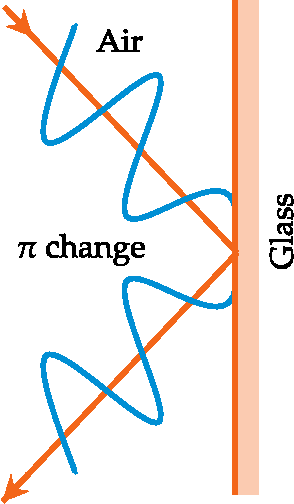
\includegraphics[height=5cm,width=4cm]{diagram-20211216(7)-crop}
		\caption{}
		\label{}
	\end{figure}
	\item A light wave travelling from a denser medium $\left(\mu_{2}\right)$ to a rarer medium $\left(\mu_{1}\right)$ does not undergo a change in phase on reflection at the boundary of denser-to-rarer medium . Therefore, the change in path is zero.
	\begin{figure}[H]
		\centering
		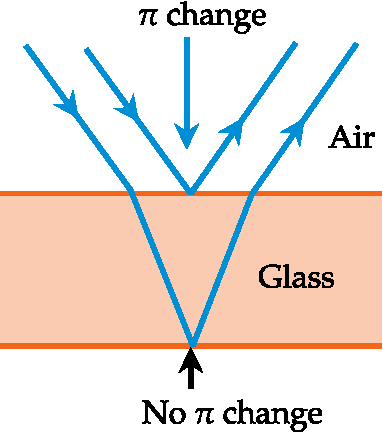
\includegraphics[height=4cm,width=5cm]{diagram-20211216(8)-crop}
		\caption{}
		\label{}
	\end{figure}
\end{enumerate}
\subsection{Superposition of waves}
When two or more wave overlaps, resultant displacement at any point and at any instant may be found by adding the instantaneous displacement that would be produced at the point by the individual waves if each were present alone.
\subsection{Interference}
If two or more lightwave of same frequency overlap at a point,the resultant effect depends on the phase of the waves as well as their amplitudes.The resultant wave at any point at any instant of time is goverened by the principle of superposition.Let us assume that the component waves are of the same amplitude\\
At certain points the two waves are in phase.The amplitude of the resultant wave will then be equal to the sum of the amplitude of the two waves.\\
\begin{figure}[H]
	\centering
	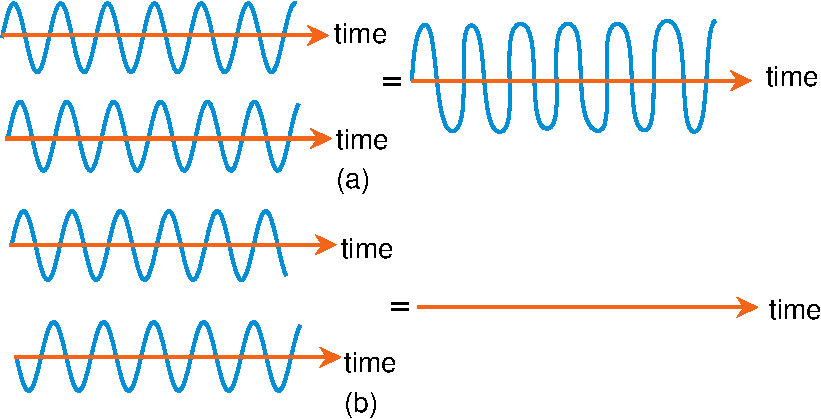
\includegraphics[height=5cm,width=8cm]{diagram-20211216(6)-crop}
	\caption{}
	\label{}
\end{figure}
$$A_R=A+A=2A$$
Intensity $$I_R\propto 2^2A^2=4I$$
But we add directly $$I_R>I+I=2I$$
Which is less than 4I\\
Interference produced at these points is known as constuctive interference.Abright band is observed at the point of constructive interference.\\
At certain points the two waves are out of phase.The amplitude of the resultant wave will then be equal to the difference of the amplitude of the two waves.\\
$$A_R=A-A=0$$
$$I_R=0$$
$$I_R<2I$$
Interference produced at these points is known as destructive interference.A dark band is observed at the point of destructive  interference.\\
When we takes the average value of the intensities of bright and dark spot,\\
$$I_R=\frac{4I+0}{2}=2I$$ Thus we got the same result $2I$.\\
\textbf{so Interference can be defined as the redistribution of light energy due to the superposition of light waves from two or more coherent sources.}\\
If the optical path difference between the two waves are zero or integral multiple of wavelength constructive interference will occur.\\
$$\Delta=m\lambda$$ where m=0,1,2,3,...\\
If the optical path difference between the two waves are odd integralof half multiple of wavelength$(\lambda/2)$ destructive interference will occur.\\
$$\Delta =(2m+1)\lambda/2$$
\subsection{Theory of interference}
Let us assume that the electric field components of the two waves rriving at point P vary with time as
$$
\text { and } \quad \begin{aligned}
&E_{A}=E_{1} \sin \omega t \\
&E_{B}=E_{2} \sin (\omega t+\delta)
\end{aligned}
$$
where $\delta$ is the phase difference between them. According to principle of superposition, the resultant electric field at the point P due to the simultaneous action of the two waves is given by
$$
\begin{aligned}
E_{R} &=E_{A}+E_{B} \\
&=E_{1} \sin \omega t+E_{2} \sin (\omega t+\delta) \\
&=E_{1} \sin \omega t+E_{2}(\sin \omega t \cos \delta+\cos \omega t \sin \delta) \\
&=\left(E_{1}+E_{2} \cos \delta\right) \sin \omega t+E_{2} \sin \delta \cos \omega t
\end{aligned}
$$
$$\begin{aligned}
&\text { Let } \quad E_{1}+E_{2} \cos \delta=E \cos \phi \\
&\text { and } \quad E_{2} \sin \delta=E \sin \phi
\end{aligned}$$
where $\mathrm{E}$ is the amplitude of the resultant wave and $\phi$ is the new initial phase angle. In order to solve for $\mathrm{E}$ and $\phi$, we square and add the above  two equations.
$$
\begin{aligned}
&\left(E_{1}+E_{2} \cos \delta\right)^{2}+E_{2}^{2} \sin ^{2} \delta=E^{2}\left(\cos ^{2} \phi+\sin ^{2} \phi\right) \\
&\text { or } \quad E^{2}=E_{1}^{2}+E_{2}^{2} \cos ^{2} \delta+2 E_{1} E_{2} \cos \delta+E_{2}^{2} \sin ^{2} \delta \\
&\text { or } \quad E^{2}=E_{1}^{2}+E_{2}^{2}+2 E_{1} E_{2} \cos \delta
\end{aligned}
$$
Thus, it is seen that the square of the amplitude of the resultant wave is not a simple sum of the squares of the amplitudes of the superposing waves, there is an additional term which is known do the interference term.
\subsection{Intensity distribution}
The intensity of light wave is given by the square of its amplitude.\\
$$I=\frac{1}{2}\epsilon_{0}cE^2\propto E^2$$
$$E^{2}=E_{1}^{2}+E_{2}^{2}+2 E_{1} E_{2} \cos \delta$$
$$I=I_{1}+I_{2}+2 \sqrt{I_{1} I_{2}} \cos \delta$$
We see that the resultant intensity at $\mathrm{P}$ on the screen is not just the sum of the intensities due , the separate waves. The term $2 \sqrt{I_{1} I_{2}} \cos \delta$ is known as the interference term. Whenever the phase difference between the waves is zero, i.e. $\delta=0$, we have maximum amount of light. Thus,
$$
I_{\max }=I_{1}+I_{2}+2 \sqrt{I_{1} I_{2}}
$$
$$\text { When } I_{1}=I_{2}=I_{\mathrm{o}} \quad I_{\max }=4 I_{o}$$
It means that the resultant intensity $I$ will be more than the sum of the intensities due to the jo sources.

When the phase difference is $\delta=180^{\circ}, \cos 180^{\circ}=-1$ and we have a minimum amount of lght.
$$
I_{\min }=I_{1}+I_{2}-2 \sqrt{I_{1} I_{2}}
$$
which, when $I_{1}=I_{2}$, becomes
$$
I_{\min }=0
$$
It means that the resultant intensity $I$ will be less than the sum of the intensities due to the two sources.
At points that lie between the maxima and minima, when $I_{1}=I_{2}=I_{0}$, we get
$$
\begin{aligned}
I &=I_{o}+I_{o}+2 I_{o} \cos \delta \\
&=2 I_{o}(1+\cos \delta)
\end{aligned}
$$
Then using the identity $1+\cos \delta=2 \cos ^{2}\left(\frac{1}{2} \delta\right)$, we get
$$
I=4 I_{o} \cos ^{2}\left(\frac{1}{2} \delta\right)
$$
\begin{figure}[H]
	\centering
	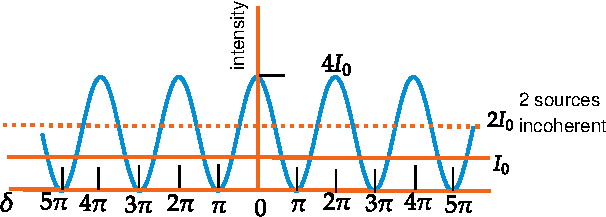
\includegraphics[height=5cm,width=10cm]{intensity-crop}
	\caption{}
	\label{}
\end{figure}
\section{Young's interference experiment}
\begin{figure}[H]
	\centering
	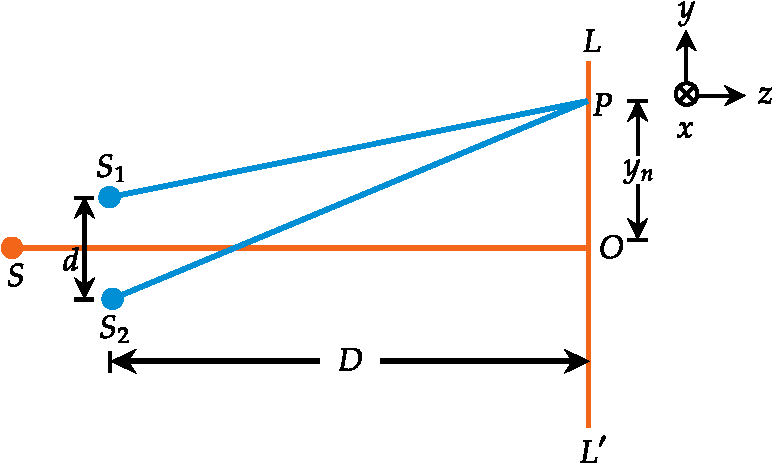
\includegraphics[height=5cm,width=8cm]{diagram-20211217(3)-crop}
	\caption{}
	\label{}
\end{figure}
Let $S_{1}$ and $S_{2}$ represent the two pinholes of the Young's interference experiment. We would determine the positions of maxima and of minima on the line $L L^{\prime}$ which is parallel to the $y$-axis and lies in the plane containing the points $S, S_{1}$ and $S_{2}$ as shown in the figure. We will show that the interference pattern (around the point $O$ ) consists of a series of dark and bright lines perpendicular to the plane of o being the foot of the perpendicular from the point $S$ on the screen.

For an arbitrary point $P$ (on the line $L L^{\prime}$ ) to correspond to a maximum we must have
$$
S_{2} P-S_{1} P=n \lambda ; n=0,1,2 \ldots
$$
$$\begin{aligned}
\left(S_{2} P\right)^{2}-\left(S_{1} P\right)^{2} &=\left[D^{2}+\left(y_{n}+\frac{d}{2}\right)^{2}\right]-\\
&\left[D^{2}+\left(y_{n}-\frac{d}{2}\right)^{2}\right] \\
&=2 y_{n} d
\end{aligned}$$
where
$$
S_{1} S_{2}=d \text { and } O P=y_{n}
$$
Thus
$$
S_{2} P-S_{1} P=\frac{2 y_{n} d}{S_{2} P+S_{1} P}
$$
$d<<<D$ S o we can replace $S_{2} P+S_{1} P=2D$\\
Then \\
$$
S_{2} P-S_{1} P=\frac{2 y_{n} d}{2D}
$$
$$S_{2} P-S_{1} P \approx \frac{y_{n} d}{D}$$
$$
S_{2} P-S_{1} P=n \lambda ; n=0,1,2 \ldots
$$
Then \\
$$y_{n}=\frac{n \lambda D}{d}$$
Thus the dark and bright fringes are equally spaced and the distance between two consecutive dark (or bright) fringes is given by
$$
\beta=y_{n+1}-y_{n}=\frac{(n+1) \lambda D}{d}-\frac{n \lambda D}{d}
$$
$$\beta=\frac{\lambda D}{d}$$
Which is the expression for the fringe width.\\
\subsubsection{Position of fringe}
\textbf{Position of nth bright fringe}\\
$$S_{2} P-S_{1} P= \frac{y_{n} d}{D}=n\lambda$$
$$y=\left( nD/d\right) \lambda$$
\textbf{Position of nth dark fringe}\\
$$S_{2} P-S_{1} P= \frac{y_{n} d}{D}=(2n-1)\lambda/2$$
$$y=\frac{(2n-1)D \lambda}{2d}$$
\begin{exercise}
	In Young's  expt, two coherent sources are placed 0.90mm apart and fringes are observed 1m away .If it produces second dark fringe at a distance of 1mm from central fringe,what would be wavelength of the monochromatic light used?
\end{exercise}
\begin{answer}
	$$y=\frac{(2n-1)D \lambda}{2d}$$
	$$\lambda=\frac{2yd}{(2n-1)D}$$
	$$\lambda=\frac{2\times 10^{-3}\times 0.9\times 10^{-3}}{(2\times 2-1)\times 1}$$
	$$\lambda=0.6\times 10^{-5}cm$$
\end{answer}
\begin{exercise}
	In a young's double slip experiment the angular width of a fringe on a distant screen is $1^{\circ}$.The wavelegth of the light used is $6280A^{\circ}$ .What is the diference between the two coherent sources.?
\end{exercise}
\begin{answer}
	The angular fringe width is given by $\alpha=\frac{\lambda}{d}$\\
	Where $\lambda$ is the wavelegth and d is the distance between two coherent sources.Thus $d=\frac{\lambda}{\alpha}$\\
	Given $\lambda=6280A^{\circ}$ $\alpha=1=\frac{\pi}{180}$
$$d=\frac{6280\times 10^{-10}}{3.14}\times 180=3.6\times10^{-5}=0.036mm$$	
\end{answer}
\begin{exercise}
	In Young's double slit experiment ,the slits are illuminated by white light.The distance between two slits d and screen is D distance from the slits .Some wavelength are missing on the screen in front of one of the slits .These wavelength are?
\end{exercise}
\begin{answer}
	\begin{figure}[H]
		\centering
		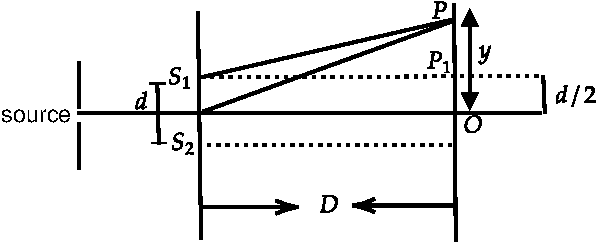
\includegraphics[height=5cm,width=8cm]{YOUNG-crop(1)}
		\caption{}
		\label{}
	\end{figure}
Path difference at any point P in front of one of the slits$=\frac{yd}{D}$\\
For missing wavelength (ie for dark fringes)\\
Path difference $=(2n-1)\lambda/2=\frac{yd}{D}$
$\implies \quad \lambda=\frac{2yd}{D(2n-1)}$\\
But $x=\frac{d}{2}$,because the point is $P_1$ where we want missing wavelength.\\
$\therefore \quad \quad \lambda=\frac{d^2}{D(2n-1)}	$\\
For n=1,2,3, etc missing wavelength are \\
$$\frac{d^2}{D},\frac{d^2}{3D},\frac{d^2}{5D},...$$
\end{answer}
\subsection{The intensity distribution}
Let $E_1$ and $E_2$ be the electric field produced at the point P by $S_1$ and $S_2$ respectevely.The fields have in general have different direction and different magnitude.However if the distance $S_1P$ and $S_2P$ are very large in comparison to the distance $S_1S_2$.The field willbe in the same direction.Thus we may write\\
$$\left.\begin{array}{l}
\mathbf{E}_{1}=\hat{\mathbf{i}} E_{01} \cos \left(\frac{2 \pi}{\lambda} S_{1} P-\omega t\right) \\
\mathbf{E}_{2}=\hat{\mathbf{i}} E_{02} \cos \left(\frac{2 \pi}{\lambda} S_{2} P-\omega t\right)
\end{array}\right\}$$
The resultant field will be given by \\
$$E=E_1+E_2$$
$$\begin{aligned}
=\hat{\mathbf{i}}[& E_{01} \cos \left(\frac{2 \pi}{\lambda} S_{1} P-\omega t\right) \\
&\left.+E_{02} \cos \left(\frac{2 \pi}{\lambda} S_{2} P-\omega t\right)\right]
\end{aligned}$$
The intensity $(I)$ will be proportional to the square of the electric field and will be given by
$$
I=K E^{2}
$$
$$\begin{aligned}
I=& K\left[E_{01}^{2} \cos ^{2}\left(\frac{2 \pi}{\lambda} S_{1} P-\omega t\right)+\right.\\
& E_{02}^{2} \cos ^{2}\left(\frac{2 \pi}{\lambda} S_{2} P-\omega t\right)+\\
& E_{01} E_{02}\left\{\cos \left[\frac{2 \pi}{\lambda}\left(S_{2} P-S_{1} P\right)\right]+\right.\\
&\left.\left.\cos \left[2 \omega t-\frac{2 \pi}{\lambda}\left(S_{2} P+S_{1} P\right)\right]\right\}\right]
\end{aligned}$$
Since frequency is changing continuously we have to take the average value .\\
$$\left\langle\cos ^{2}(\omega t-\theta)\right\rangle=\frac{1}{2}$$
The factor $\cos(2\omega t-\phi)$ will oscillate between +1 and -1 and its average will be zero .So intensity can be written as\\
$$I=I_1+I_2+2\sqrt{I_1I_2}\cos \delta$$
Where $$\delta=\frac{2\pi}{\lambda}(S_2P-S_1P)$$
Represents the phase differnce between the displacements reaching the points P from $S_1$ and $S_2$
$$I_1=\frac{1}{2}KE_{01}$$
Represents the intensity produced by the source $S_1$ if no light from $S_2$ is allowed to fall on the screen.\\
\begin{note}
	\begin{enumerate}
		\item The maximum and minimum value of $\cos\delta$ are +1 and -1 respectevely;
		Such that maximum and minimum value of I are given by \\
		$$I_{max}=(\sqrt{I_1}+\sqrt{I_2})^2$$\\
		$$I_{min}=(\sqrt{I_1}-\sqrt{I_2})^2$$
		The maximum intensity occures when \\
		$$\delta =2n\pi \hspace{0.5cm} n=0,1,2,3...$$
		or $$S_2P-S_1P=n\lambda$$
		The minimum intensity occures when 
		$$\delta=(2n+1)\pi;n=0,1,2,3...$$
		or
		$$S_2P-S_1P=\left( n+1/2\right) \lambda$$ 
		Notice that when $I_1=I_2$ The intensity minimum is zero.In general $I_1\neq I_2$ and the minimum intensity is not zero.     
		\item If the two light sources are illuminated by different type of sources then the phase difference will vary with time in a random manner Then the average over the $\cos \theta$ will be zero.\\
		$$\left\langle\cos (\delta)\right\rangle=0$$ 
		and we obtain \\
		$$I=I_1+I_2$$
		Thus for two incoherent sources ,the resultant intensity is the sum of intensities produced bt each one of the sources independently and no interference pattern is observed.
		\item If the distances $S_1P$ and $S_2P$ are extremely large in comparison to d then\\
		$$I_1=I_2=I_0$$
		and $$I=2I_0+2I_0\cos \delta=4I_0\cos^2(\delta/2) $$ 
		The intensity vs phase difference can be plot which is same as figure(2.6) 
		\begin{figure}[H]
			\centering
			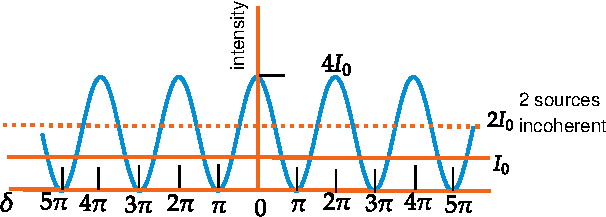
\includegraphics[height=5cm,width=10cm]{intensity-crop}
			\caption{}
			\label{}
		\end{figure}
	\end{enumerate}
\end{note}
\begin{exercise}
	Two beams of light having intensities I and 4I interfere to produce a fringe pattern on a screen.The phase difference between the beam is $\pi/2$ at a point A and $\pi$ at a point B.Then find the difference between the resultant intensities at A and B?
\end{exercise}
\begin{answer}
Here $I_1=I;I_2=4I;\theta_{1}=\pi/2;\theta_{2}=\pi$\\
$$I_A=I_1+I_2+2\sqrt{I_1I_2}\cos \theta_{1}$$
$$=I+4I+2\sqrt{I\times 4I}\cos\pi/2=51I$$
$$I_B=I+4I+2\sqrt{I\times 4I}\cos\pi=I$$
$$\therefore I_A-I_B=5I-I=41$$	
\end{answer}
\begin{exercise}
	In Young's experiment,the interference pattern is found to have an intensity ratio between the bright and dark fringes as 9.What is the ratio of (a) Intensities\\
	(b)Amplitude of the two interfering waves?
\end{exercise}
\begin{answer}
	In case of interference $$I=I_1+I_2+2\sqrt{I_1I_2}\cos \theta_{1}$$
	For I to be maximum and minimum $\cos\phi$ is 1 and -1 respectively.ie\\
	$$I_{max}=(\sqrt{I_1}+\sqrt{I_2})^2$$
	$$I_{max}=(\sqrt{I_1}-\sqrt{I_2})^2$$
	$$\frac{I_{max}}{I_{min}}=\frac{(\sqrt{I_1}+\sqrt{I_2})^2}{(\sqrt{I_1}-\sqrt{I_2})^2}=9$$
$$\frac{I_{max}}{I_{min}}=\frac{(\sqrt{I_1}+\sqrt{I_2})}{(\sqrt{I_1}-\sqrt{I_2})}=3$$
By comonendo and dividento,\\
$$\frac{\sqrt{I_1}}{\sqrt{I_2}}=\frac{3+1}{3-1}=4$$	
(b)$$\frac{I_1}{I_2}=\left[ \frac{A_1}{A_2}\right] ^2$$
$$\left[ \frac{A_1}{A_2}\right] ^2=4$$
$$\frac{A_1}{A_2}=2$$
\end{answer}
\begin{exercise}
	In Young's double slit experiment,one of the slit is wider than the other,so that amplitude of light from one slit double of that from the other slit.If $I_m$ be the maximum intensity, the resultant intensity I when they interfere at phase difference $\phi$ is given by? 
\end{exercise}
\begin{answer}
	let $a_1=a,I_1=a_1^2=a^2$\\
	$a_2=2a,I_2=a_2^2=4a^2$\\
	$I_2=2I_1$\\
	$I_r=a_1^2+a_2^2+2a_1a_2\cos\phi$\\
	$=I_1+I_2+2\sqrt{I_1I_2}\cos\phi$\\
	$I_r=I_1+4I_1+2\sqrt{4I_1^2}\cos\phi$\\
	$\implies =5I_1+4I_1\cos \phi$\\
	$I_{max}=(a_1+a_2)^2=(a+2a)^2=9a^2$\\
	$I_{max}=9I_1\implies\frac{I_{max}}{9}$\\
	Substituting the value in $I_R$\\
	$I_r=\frac{5I_{max}}{9}+\frac{4I_{max}}{9}\cos\phi$\\
	$I_r=\frac{I_{max}}{9}\left[ 5+4\cos\phi\right] $\\
	$I_r=\frac{I_{max}}{9}\left[ 5+8\cos^2\phi/2-4\right] $\\
	$I_r=\frac{I_{max}}{9}\left[ 1+8\cos^2\phi/2\right] $
\end{answer}
\begin{exercise}
	Let the intensity on the screen at a point  P in double slit interference pattern be $60\%$ of the maximun value?
	(a)What is the minimum phase difference between the sources?
	(b)What is the corresponding path difference if the wavelength of light is $\lambda=500nm$
\end{exercise}
\begin{answer}
(a)	The intensity $I=I_{max}\cos^2\left( \delta/2\right) $\\
 0.60=$\cos^2\left( \delta/2\right) $\\
 $\delta=78.5^{\circ}=1.37rad$\\
 (b)The phase difference $\delta$ is related to the path difference$\Delta$ by the relation\\
 $\Delta=\frac{\lambda \delta}{2\pi}=109nm$
\end{answer}
\subsection{Interference with white light}
When the slit is illuminated by white light,the central fringe produced at the point 0 will be white because all the wavelength will constuctvely interfere here.Now slightly bellow and above the point 0 the fringes will be coloured.The coloured fringes will soon disappear because at points far away from 0 there will be so many wavelength will constructively interferethat we will observe uniform white illumination.
\subsection{Displacement of fringes}
\begin{figure}[H]
	\centering
	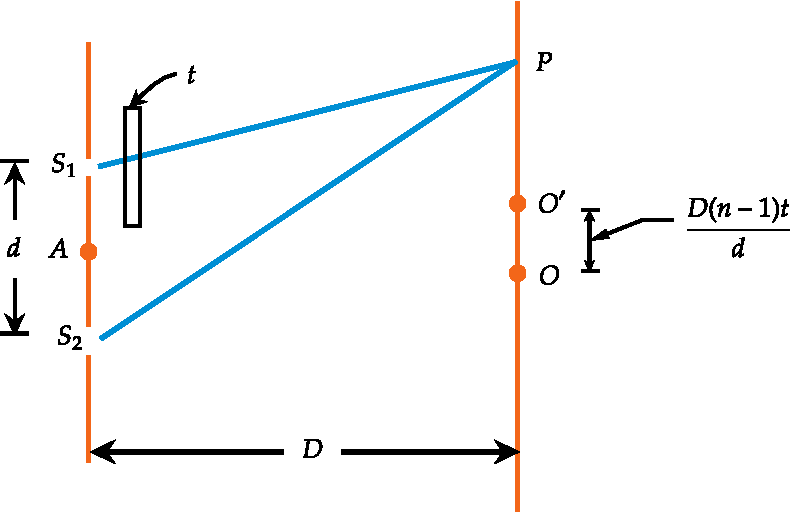
\includegraphics[height=5cm,width=8cm]{diagram-20211217(16)-crop}
	\caption{}
	\label{}
\end{figure}
We will now discuss the change in the interference pattern produced by introducing a thin transparent plate in the path of one of the two interference beams . Let $t$ be the thickness of the plate and let $n$ be its refractive index. It is easily seen from the figure that light reaching the point $P$ from $S_{1}$ has to traverse a distance $t$ in the plate and a distance $S_{1} P-t$ in air. Thus the time required for the light to reach from $S_{1}$ to the point $P$ is given by\\
$$\begin{aligned}
\frac{S_{1} P-t}{c}+\frac{t}{v} &=\frac{1}{c}\left[S_{1} P-t+n t\right] \\
&=\frac{1}{c}\left[S_{1} P+(n-1) t\right]
\end{aligned}$$
Where c is the speed of the light.equation shows that by introducing thin plate the effective optical path will increases by $(n-1)t$.Thus whwn the thin plate is introduced the central fringe will be formed at $0^{\prime}$.Where\\
$$S_{1} O^{\prime}+(n-1) t=S_{2} O^{\prime}$$
Since $$S_2O^{\prime}-S_1O^{\prime}=\frac{d}{D}OO^{\prime}$$
Therefore \\
$$(n-1)t=\frac{d}{D}OO^{\prime}$$
$$OO^{\prime}=\frac{D(n-1)t}{d}$$
Usually denoted by\\
$$\Delta=\frac{D(n-1)t}{d}$$
The above principle enable us to determine the thickness of the extremely thin transparent sheets.
\begin{exercise}
	In a double slit interference arrangement one of the slit is covered by a thin mica sheet whose refeactive index is 1.58.The distance $S_1S_2$ and AO are 0.1cm and 50cm respectively .Due to the introduction of the mica sheet the central fringe shifted by 0.2cm.Determine the thickness of the mica sheet.
\end{exercise}
\begin{answer}
$\Delta=0.2cm;d=0.1cm;D=50cm$\\
$$t=\frac{d\Delta }{D(n-1)}=\frac{0.1\times 0.2}{50\times 0.58}=6.7\times 10^{-4}$$
\end{answer}
\section{Thin film interference}
In thin film interference pattern will obtain by the division of amplitude;For example if a plane wave falls on a thin film then the wave reflected from the upper surface interfere with the wave reflected from the lower surface.
\subsection{Interference by a plane parallel film when illuminated by a plane wave}

($\textbf{I}$) 
\begin{figure}[H]
	\centering
	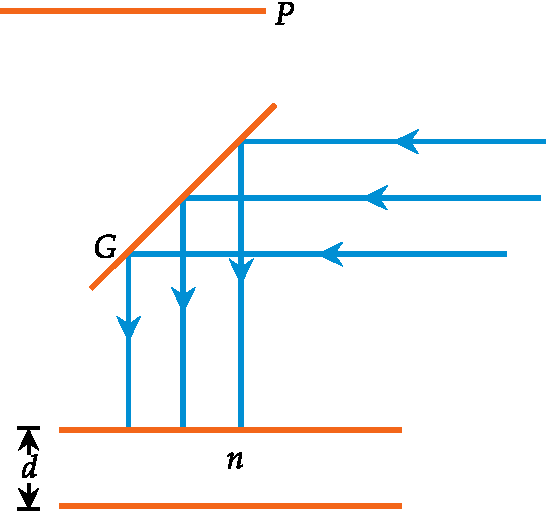
\includegraphics[height=5cm,width=8cm]{diagram-20211217(14)-crop}
	\caption{}
	\label{}
\end{figure}
If a plane wave is incident normally on a thin film of uniform thickness d then the wave reflected from the upper surface interfere with the wave reflected from the lower surface.If d is the seperation between the parallel plane and n is the refractive index of the medium.Then the path difference between the two wave will be $2nd$.\\
Condition for constructive interference 
$$2nd=\left( m+12\right)\lambda $$
Because there is a phase change of $\pi$ occur at the air to upper plane interface.\\
The condition for distructive interference\\
$$2nd=m\lambda$$
($\textbf{II}$) It may be noted that the amplitude of the wave reflected from upper and lower surface will in general be slightly different and as such the interference will not be completely distructive.By the appropriate choice of refractive index of the media II and III the amplitude can be mad every equal.\\
\begin{figure}[H]
	\centering
	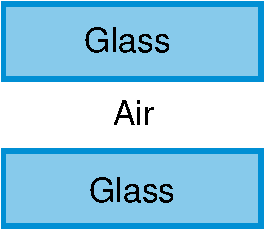
\includegraphics[height=3cm,width=4cm]{diagram-20211217(19)-crop}
	\caption{}
	\label{}
\end{figure}
There  is a phase change occur at air to glass interface and no  phase change at glass air surface.\\
so condition for interference become\\
Condition for constructive interference 
$$2nd=\left( m+1/2\right)\lambda $$
The condition for distructive interference\\
$$2nd=m\lambda$$
($\textbf{III}$) Suppose the I medium is a crown glass(n=1.52), the medium II is a oil of refractive index 1.60 and the medium III flint glass (n=1.66) Then a phase change of $\pi$ will occur at the both the reflections and the conditions for maxima and minima would be \\
$$2nd=\left( m+1/2\right)  \quad \quad \text{ minima } $$ 
$$2nd=m\lambda \quad \quad \text{maxima }$$
In general whenever the refractive index of the second medium is in between the refractive indices of the first and third then the condition of the maxima and minima will be like this.\\
\textbf{(IV)}
\begin{figure}[H]
	\centering
	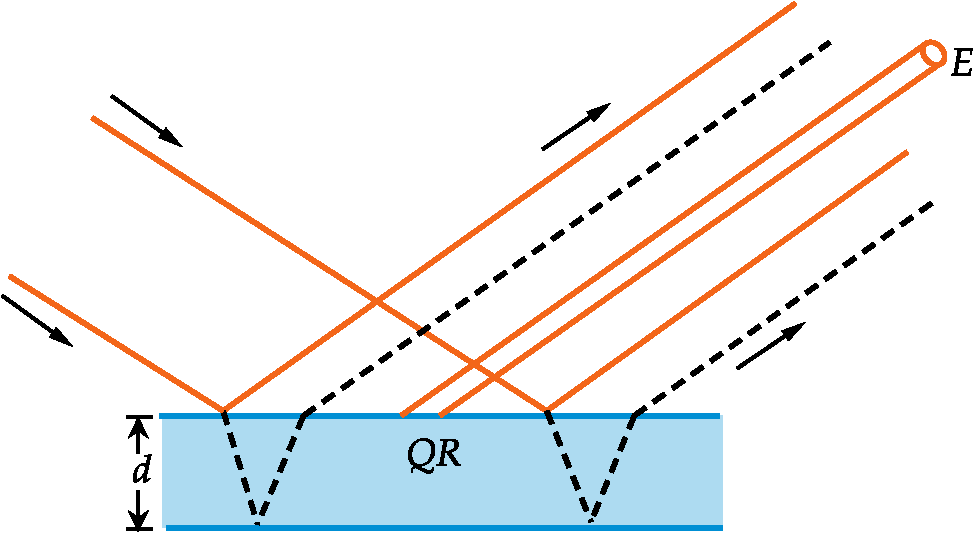
\includegraphics[height=4cm,width=8cm]{diagram-20211218(1)-crop}
	\caption{}
	\label{}
\end{figure}
Consider the oblique incidence of the plane wave on a thin film .Here also the wave reflected from the upper surface of the film interfere with the wave reflected from the lower surface of the film.The latter traverse an additional optical path $\Delta$ which is given by \\
$$\Delta=2n_2d\cos \theta^{\prime} \quad \text{ (The cosine law)}$$
Where $\theta^{\prime}$  is the angle of refraction.\\
now the  condition for interference become\\
Condition for constructive interference 
$$2n_2d\cos \theta^{\prime}=\left( m+1/2\right)\lambda $$
The condition for distructive interference\\
$$2n_2d\cos \theta^{\prime}=m\lambda$$
\subsection{Non reflecting films}
One of the important applications of the thin film interference lies in reducing the reflectivity of the lens surfaces.When a light beam is incident normally on a dielectric of refractive index $n_2$ then the amplitudes of the reflected and transmitted waves are related to that of the incident beam through the following relations\\
$$a_r=\frac{n_1-n_2}{n_1+n_2}a_i$$
$$a_t=\frac{2n_1}{n_1+n_2}a_i$$
Where $a_i$ $a_r$ and $a_t$ are the amplitude of the incident beam,reflected beam and transmitted beam respectvely.\\
Notice that when $n_2>n_1$ $a_r$ is negative showing that when a reflection occurs at a denser medium a phase change of $\pi$ occurs.
\begin{figure}[H]
	\centering
	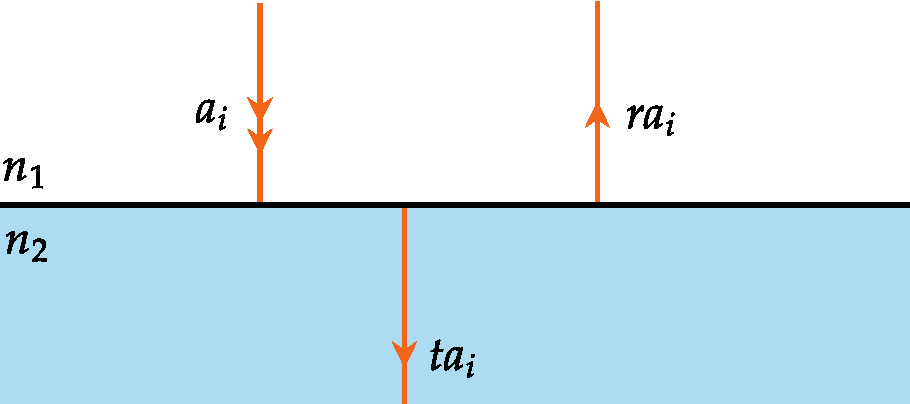
\includegraphics[height=3cm,width=5cm]{diagram-20211218-crop}
	\caption{}
	\label{}
\end{figure}
The amplitude of the reflection and transmisssion coefficient r and t are therefore given by\\
$$r=\frac{n_1-n_2}{n_1+n_2}$$
$$t=\frac{2n_1}{n_1+n_2}$$
It is interesting to point out that if $r^{\prime}$ and $t^{\prime}$ are the reflection and transmission coefficients where light propagating in a medium of refractive index $n_2$ is incident on a medium of refractive index $n_1$
$$r^{\prime}=\frac{n_2-n_1}{n_2+n_1}=-r$$
$$t^{\prime}=\frac{2n_2}{n_1+n_2}$$
and 
$$1-tt^{\prime}=1-\frac{4n_1n_2}{(n_1+n_2)^2}=\left( \frac{n_1-n_2}{n_1+n_2}\right) ^2=r^2$$

\paragraph{Application}
\begin{figure}[H]
	\centering
	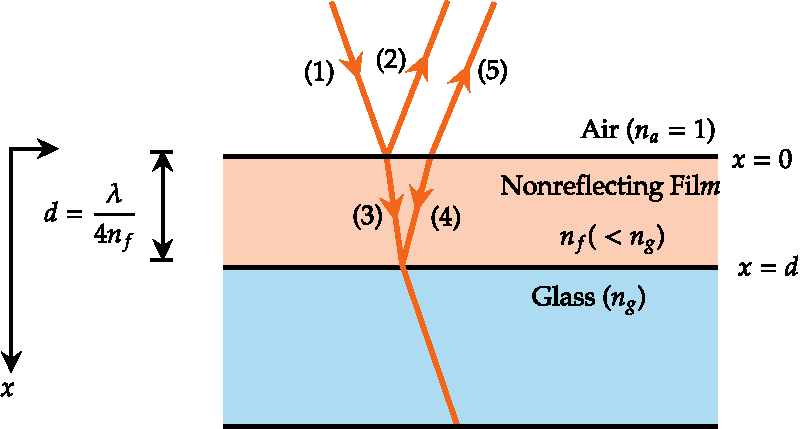
\includegraphics[height=5cm,width=10cm]{diagram-20211218(2)-crop}
	\caption{}
	\label{}
\end{figure}
for near normal incidence,the reflectivity of crown glass surface in air is
$$
\left(\frac{n-1}{n+1}\right)^{2}=\left(\frac{1.5-1}{1.5+1}\right)^{2} \simeq 0.04
$$
i.e., $4 \%$ of the incident light is reflected. For a dense flint glass $n \simeq 1.67$ and about $6 \%$ of light is reflected. Thus, if we  have a large number of surfaces, the losses at the interfaces can be considerable. In order to reduce these losses, lens surfaces are often coated with a $\lambda / 4 n$ thick 'non-reflecting film'; the refractive index of the film being less than that of the lens. For example, glass $(n=1.5)$ may be coated with an $\mathrm{MgF}_{2}$ film and the film thickness $d$ should be such that\\
$$2n_fd=\frac{1}{2}\lambda$$
$$d=\frac{\lambda}{4n_f}$$
\begin{note}
	\begin{enumerate}
		\item If the refractive index of the coating film is $n_f$ ,and the first medium is air, and the refractive index of the glass is $n_g$ then we can write 
		$$ n_f=\sqrt{n_gn_a}$$
		\item Refractive indices of\\
		(a)Dense flint glass $n_g=1.29 \quad n_f=1.29$\\
		(b)lihgt crown glass $n_g=1.5 \quad n_f=1.22$
		\item Refractive indices of \\
		(a)Magnesium fluride $n_f=1.38$\\
		(b)Cryolite $n_f=1.36$
		\item For a $\frac{\lambda}{4n}$ thick film the reflectivity will be about 
		$$\left[ \frac{n_f-n_a}{n_f+n_a}-\frac{n_g-n_f}{n_g+n_f}\right] ^2$$
		For $n_a=1$, $n_f=1.38$ and $n_g=1.5$ the reflectivity will be about $1.3\%$.In the absence of the film the reflectivity would have been about $4\%$.\\
		The technique of reducing reflectivity is known as blooming.
	\end{enumerate}
\end{note}
\subsection{High reflectivity by thin film deposition}
Another important application of the thin film interference is the high reflectivity by thin film deposition .The glass surface is coated with a thin film of suitable material to increase the reflectivity.The thin film thickness is again $\frac{\lambda}{4n_f}$ where $n_f$ represents the refractive index of the film ;however the film is such that its refractive index is greater than that of the glass ;consequently an abrupt phase change of $\pi$ occurs only at the air film interface  and the beam reflected from the air film interface and the film glass interface constructiveley interfere.The reflectivity up to $35\%$ can be increased bt this technique.
\subsection{Interference by a film with two non parallel reflecting surface}
Now we discuss the interference pattern produced by a film of varying thickness.Such a film may be produced by a wedge which consisit of two non parallel plane surfaces.\\
There are  two cases,first we consider a parallel beam of light incident normally on the upper surfaces of the film.Second on the other hand using a point source.\\
\textbf{CASE I}\\
\begin{figure}[H]
	\centering
	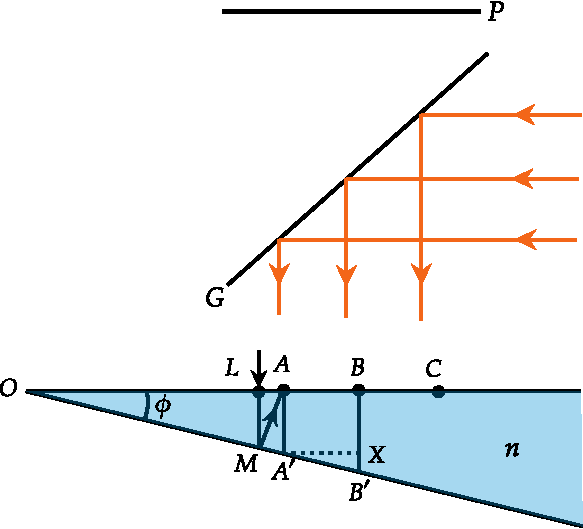
\includegraphics[height=8cm,width=8cm]{diagram-20211218(6)-crop}
	\caption{}
	\label{}
\end{figure}
Consider the first case as shown in the figure .a plane parallel beam illuminates the upper surfaces of the film.A photographic plate will record the straight line interference fringes which will be parallel to the edge of the The dots in the figure indicated the the position of maxima.\\
In order to find the distance between two consecutive fringes on the film  we not that for a point  A to be bright\\
$$ n(LM+MA)=\left( m+1/2\right) \lambda ; m=0,1,2,....$$
However the wedge angle $\phi$ is very small $$LM+MA=2AA^{\prime}$$
where $A A^{\prime}$ represents the thickness of the film at $A$. Thus the condition for the point $A$ to be bright is
$$
2 n A A^{\prime} \approx\left(m+\frac{1}{2}\right) \lambda
$$
Similarly, the next bright fringe will occur at the point $B$ where
$$
2 n B B^{\prime} \approx\left(m+\frac{3}{2}\right) \lambda
$$
$$\begin{aligned}
&\text { Thus } \quad 2 n\left(B B^{\prime}-A A^{\prime}\right) \approx \lambda \\
&\text { or } \quad X B^{\prime} \approx \lambda / 2 n \\
&\text { But } \quad X B^{\prime}=\left(A^{\prime} X\right) \tan \phi \\
&\text { or } \quad A^{\prime} X=\beta \approx \frac{\lambda}{2 n \phi}
\end{aligned}$$
where $\beta$ represents the fringe width and we have assumed $\phi$ to be small. Such fringes are commonly referred to as fringes of equal thickness.\\
\textbf{CASE II}\\
\begin{figure}[H]
	\centering
	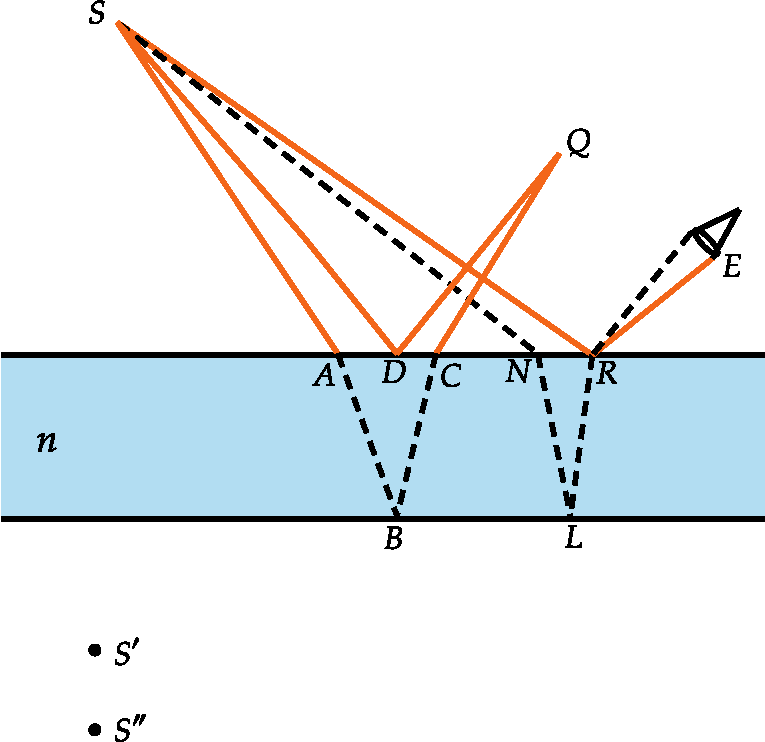
\includegraphics[height=6cm,width=8cm]{diagram-20211218(7)-crop}
	\caption{}
	\label{}
\end{figure}
On the other hand, for a point source, the fringe pattern will be similar to the parallel film case; i.e., for near normal incidence, the pattern will be very nearly the same as produced by two sources $S^{\prime}$ and $S^{\prime \prime}$ \\
The intensity of an arbitrary point $Q$ will be determined by the following equations:
$$[S A+n(A B+B C)+C Q]-[S D+D Q]$$
$$\begin{aligned}
&=\left(m+\frac{1}{2}\right) \lambda \text { maxima } \\
&=m \lambda \quad \text { minima }
\end{aligned}$$
If we view the film with naked eye (say at the position $E$ - then only a small portion of the film (around the point $R$ ) would be visible and the point $R$ will be bright or dark as the optical path difference $[\{S N+n(N L+$ $L R)\}-S R]$ is $\left(m+\frac{1}{2}\right) \lambda$ or $m \lambda$ respectively. 
\paragraph{Colours of thin films}
We have seen in the previous section that if light from an extended monochromatic source (like a sodium lamp) is incident normally on a wedge, then equally spaced dark and bright fringes will be observed. The distance between two consecutive bright (or dark) fringes is determined by the wedge angle, the wavelength of light and by the refractive index of the film. If we use a polychromatic source (like an incandescent lamp) we will observe coloured fringes. Further, if instead of a wedge we have a film of arbitrarily varying thickness we will again observe fringes, each fringe representing the locus of constant film thickness This is indeed what we see when sunlight falls on a soap bubble or on a thin film of oil on water; It should be mentioned that if the optical path difference between the waves reflected from the upper surface of the film and from the lower surface of the film should be comparable with that of the wavelength used.
\section{Newton's rings}
\begin{figure}[H]
	\centering
	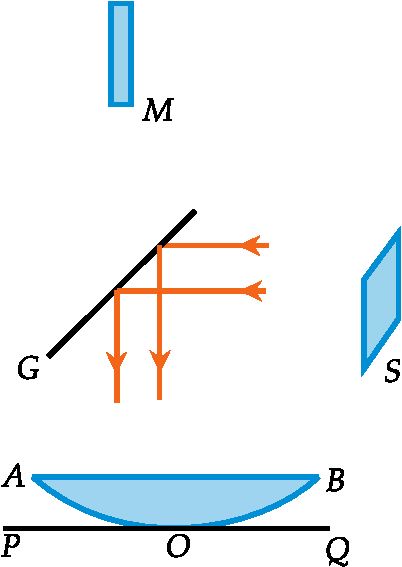
\includegraphics[height=5cm,width=5cm]{diagram-20211218(9)-crop}
	\caption{}
	\label{}
\end{figure}
If we place a plano-convex lens on a plane glass surface,a thin film of air is formed between the curves surface of the lens(AOB) and the plane glass plate (POQ).Thickness of the air film is zero at the point of contact 0 and increases as one move away from the point of contact.If we allow monochromatic light to fall on a surface of the lens then the two reflected light from each surface interfere.For near normal incidence the optical path difference between the two wave is very nearly equal to 2nt.\\
Where n is the refractive index of the film \\
t is the thickness of the film.\\
Thus whenever the thickness of the airfilm of the airfilm satisfies the condition.\\
$$2nt=\left( m+1/2\right) \lambda;m=0,1,2,3....$$we will have maxima.similarly the condition\\
$$2nt =m\lambda$$ will corresponds to minima.\\
Since the convex side of the lens is a sperical surface the thickness of the air film will be constant over a circle (whose centre will be at $O$ ) and we will obtain concentric dark and bright rings. These rings are known as Newton's rings.\\
\textbf{Radii of the rings}\\
\begin{figure}[H]
	\centering
	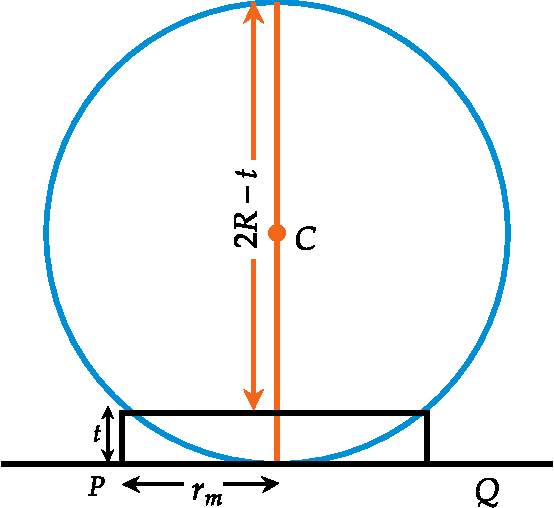
\includegraphics[height=5cm,width=5cm]{diagram-20211218(8)-crop}
	\caption{}
	\label{}
\end{figure}
the thickness of the air film will be constant over a circle whose center is at the point of contact $0 .$ Let the radius of the $m$ th dark ring be $r_{m}$ and if $t$ is the thickness of the air film where the $m$ th dark ring appears to be formed, $$r_{m}^{2}=t(2 R-t)$$
Where R is the radius curvature of the lens. Since tha value t is very small compared to R we can nglect it.Then we obtain\\
$$\begin{aligned}
r_{m}^{2} &=2 R t \\
2 t & \approx \frac{r_{m}^{2}}{R}
\end{aligned}$$
substituting in $2nt=m\lambda$ \\
$$r_{m}^{2} \approx m \lambda R ; m=0,1,2, \ldots$$
Which implies that the radius of the rings varies as square root of the natural numbers.\\
Between two dark rings there will be bright ring whose radius will be $$\sqrt{m+1/2}\lambda R$$
\paragraph{Determination of wavelength}
While carrying out the experiment one should measure the radiiof the $m^{{th}}$ and (m+p)th ring(p=10) and take the difference in the squres of the radii($r^2_{m+p}-r_m^2=p\lambda R$) which is indeed independent of m.In terms of diameter the wavelength is given by the following expression \\
$$\lambda=\frac{D^2_{m+p}-D^2_m}{4pR}$$
If radius R is known wavelength can be easily found.\\
\begin{note}
	\begin{enumerate}
		\item The central spot will be dark.
		\item The spacing between two dark rings goes on decreasing when we move  from center to the periphery.
		\item If the refractive index of n is introduced between the lens and the glass plate the radii of thee dark rings would be given by
		$$ r_m=(m\lambda R/n)^{1/2}$$
		\item If the refractive index of the material of the lens and of the glass plate are different and if the refractive index of the liquid lies between the two values,the central spot will be bright and the equation of radii would give the radii of the bright fringes.
	\end{enumerate}
\end{note}
\section{Coherence}
If we consider two waves of same frequency ,they may differ in amplitude but they maintain a predictable phase relationship.The difference in their phases may have any value from zero radians to a maximum of 2$\pi$ radians;but the phase difference remains the constant.Thus two or more waves of the same frequency can maintain the same phase or constant phase difference over a distance and time  is called a \textbf{coherent} wave\\
If one or both of the waves undergoes change in frequency irregularly .Under these conditions thsese waves are said to be incoherent. The light emitted by most of the light sources is \textbf{incoherent} as the frequency of light changes abruptly and irregularly.\\
\textbf{Proof}\\
Let the displacement produced by the sources $S_1$ and $S_2$ be given by \\
$$y_1=a\cos \omega t$$
$$y_2=a\cos (\omega t+\phi)$$
Then the resultant displacement would be 
$$y=y_1+y_2=2a\cos \phi/2\cos (\omega t+\phi/2)$$
The intensity(I)  which is preportional to the square of the amplitude can be written in the form\\
$$I=4I_0\cos^2 \phi/2$$
Where $I_0$ is the intensity produced by each one of the sources individually.Clearly if $\phi=\pm \pi ,\pm 3\pi,...$ the resultant intensity will be zero. and we will have minima.On the other hand $\phi=0,\pm2\pi,\pm 4\pi,...$ the intensity will be maxima ($=4I_0$).\\
However if the phase difference($\phi$) between the sources $S_1$ and $S_2$ is changing with time ,the observed intensity will be given by 
$$I=4I_0\langle \cos^2\phi/2\rangle$$
But $\langle\cos^2\phi/2\rangle=1/2$
Then \\
$$I=2I_0$$
Which implies that if the sources are coherent then the resultant intensity is the sum of two intensities$(I_0+I_0=2I_0)$ there is no interference.\\
\begin{enumerate}
	\item \textbf{Temperal coherence}\\
	 A light wave is produced when an excited atom goes to the ground state and emit light.\\
	 (i) Duration of this transition is about $10^{-9}$ to $10^{-10}$ seconds .Thus the emitted wave remains sinusoidal for this much time.\\This time is known as coherence time.$(\tau_c)$\\
	 (ii)DEfinite phase relationship is maintained for a length $L=c\tau_c$ called coherence length.\\\\
	 For neon $\lambda=6238 A^{\circ}$, $\tau_c=10^{-10} sec$ and L=0.03m.\\
	 (iii) The spectral line width $\Delta \lambda$ is related to the coherence length L and coherence time $\tau_c$
	 $$\Delta\lambda\approx\frac{\lambda^2}{c\tau_c} \quad or \Delta\lambda\approx\frac{\lambda^2}{L}$$
	 \item \textbf{ Spatial coherence}
	 Two points in space are said to be spatially coherence if the waves reaching there maintains a constant phase difference.The points Q  and P are at the same distance from S.They will always having the same phase.Points P and $P^{\prime}$ will be spatially coherent if the distance between $P$ and $P^{\prime}$  will be spatially coherent if the distance the P nad $P^{\prime}$ much less than the coherence length ie $$PP^{\prime}<<c\tau_c$$
\end{enumerate}




\newpage
\begin{abox}
	Practice set 1 
	\end{abox}
\begin{enumerate}
	\begin{minipage}{\textwidth}
		\item In a Young's double slit interference experiment, the slits are at a distance $2 L$ from each other and the screen is at a distance $D$ from the slits. If a glass slab of refractive index $\mu$ and thickness $d$ is placed in the path of one of the beams, the minimum value of $d$ for the central fringe to be dark is
		\exyear{NET DEC 2011}
	\end{minipage}
	\begin{tasks}(2)
		\task[\textbf{A.}] $\frac{\lambda D}{(\mu-1) \sqrt{D^{2}+L^{2}}}$
		\task[\textbf{B.}] $\frac{\lambda D}{(\mu-1) L}$
		\task[\textbf{C.}]$\frac{\lambda}{(\mu-1)}$
		\task[\textbf{D.}]$\frac{\lambda}{2(\mu-1)}$
	\end{tasks}
\begin{minipage}{\textwidth}
	\item Consider the interference of two coherent electromagnetic waves whose electric field vectors are given by $\vec{E}_{1}=\hat{i} E_{0} \cos \omega t$ and $\vec{E}_{2}=\hat{j} E_{0} \cos (\omega t+\varphi)$ where $\varphi$ is the phase difference. The intensity of the resulting wave is given by $\frac{\varepsilon_{0}}{2}\left\langle E^{2}\right\rangle$, where $\left\langle E^{2}\right\rangle$ is the time average of $E^{2}$. The total intensity is
	\exyear{NET JUNE 2012}
\end{minipage}
\begin{tasks}(2)
	\task[\textbf{A.}] 0
	\task[\textbf{B.}]$\varepsilon_{0} E_{0}^{2}$
	\task[\textbf{C.}] $\varepsilon_{0} E_{0}^{2} \sin ^{2} \varphi$
	\task[\textbf{D.}] $\varepsilon_{0} E_{0}^{2} \cos ^{2} \varphi$
\end{tasks}
\begin{minipage}{\textwidth}
	\item A parallel beam of light of wavelength $\lambda$ is incident normally on a thin polymer film with air on both sides. If the film has a refractive index $n>1$, then second-order bright fringes can be observed in reflection when the thickness of the film is
	\exyear{NET DEC 2014}
\end{minipage}
\begin{tasks}(2)
	\task[\textbf{A.}] $\lambda / 4 n$
	\task[\textbf{B.}]$\lambda / 2 n$
	\task[\textbf{C.}]$3 \lambda / 4 n$
	\task[\textbf{D.}] $\lambda / n$
\end{tasks}
\begin{minipage}{\textwidth}
	\item A screen has two slits, each of width $w$ with their centres at a distance $2 w$ apart. It is illuminated by a monochromatic plane wave travelling along the $x$-axis.
	The intensity of the interference pattern, measured on a distant screen, at an angle
	$\theta=\frac{n \lambda}{w} \text { to the } x \text {-axis is }$
	\exyear{NET DEC 2016}
	\begin{figure}[H]
		\centering
		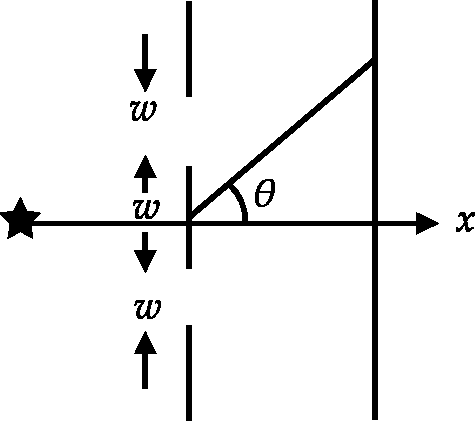
\includegraphics[height=4cm,width=5cm]{diagram-20211011(45)-crop(1)}
		\caption{}
		\label{}
	\end{figure}
\end{minipage}
\begin{tasks}(2)
	\task[\textbf{A.}] zero for $n=1,2,3 \ldots$ 
	\task[\textbf{B.}]maximum for $n=1,2,3 \ldots$
	\task[\textbf{C.}]maximum for $n=\frac{1}{2}, \frac{3}{2}, \frac{5}{2} \ldots$
	\task[\textbf{D.}]zero for $n=0$ only
\end{tasks}
\begin{minipage}{\textwidth}
	\item A pair of parallel glass plates separated by a distance $d$ is illuminated by white light as shown in the figure below. Also shown in the graph of the intensity of the reflected light $I$ as a function of the wavelength $\lambda$ recorded by a spectrometer.
	\begin{figure}[H]
		\centering
		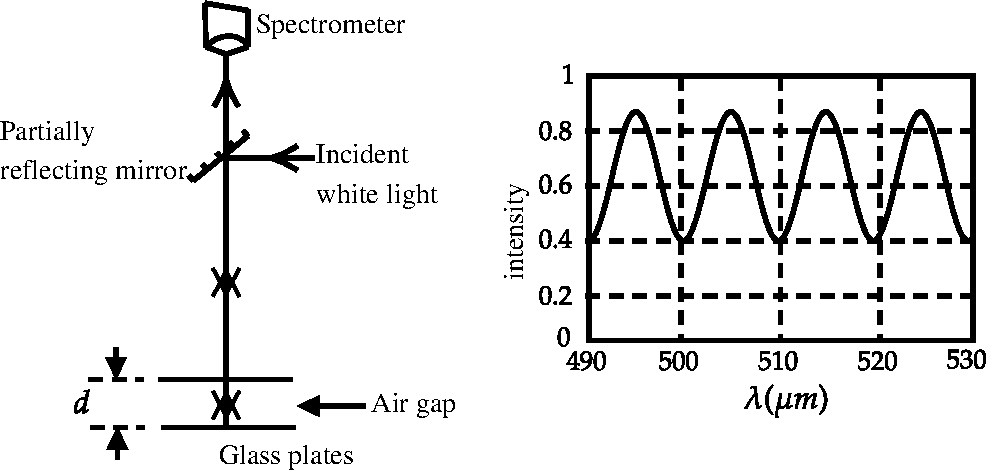
\includegraphics[height=4cm,width=8cm]{diagram-20211011(48)-crop}
	\end{figure}
	Assuming that the interference takes place only between light reflected by the bottom surface of the top plate and the top surface of bottom plate, the distance $d$ is closest to
	\exyear{NET DEC 2016}
\end{minipage}
\begin{tasks}(2)
	\task[\textbf{A.}] $12 \mu \mathrm{m}$
	\task[\textbf{B.}] $24 \mu m$
	\task[\textbf{C.}] $60 \mu m$
	\task[\textbf{D.}] $120 \mu \mathrm{m}$
\end{tasks}
\begin{minipage}{\textwidth}
	\item The figure describes the arrangement of slits and screens in a Young's double slit experiment. The width of the slit in $S_{1}$ is $a$ and the slits in $S_{2}$ are of negligible width.
	
	If the wavelength of the light is $\lambda$, the value of $d$ for which the screen would be dark is
	\exyear{NET JUNE 2017}
	\begin{figure}[H]
		\centering
		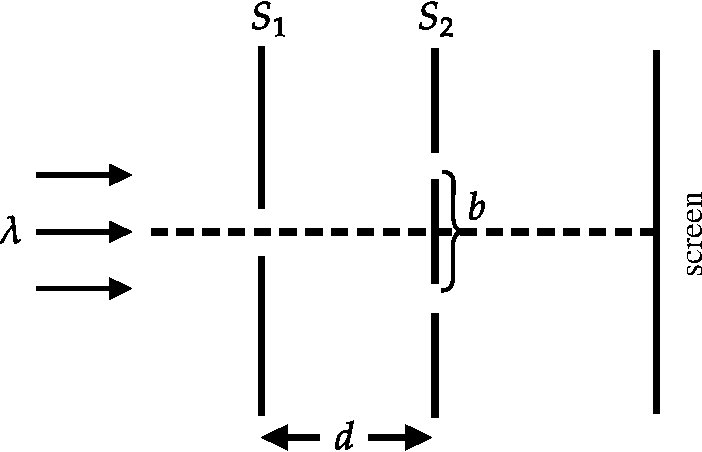
\includegraphics[height=4cm,width=6cm]{diagram-20211011(52)-crop}
	\end{figure}
\end{minipage}
\begin{tasks}(2)
	\task[\textbf{A.}] $b \sqrt{\left(\frac{a}{\lambda}\right)^{2}-1}$
	\task[\textbf{B.}]$\frac{b}{2} \sqrt{\left(\frac{a}{\lambda}\right)^{2}-1}$
	\task[\textbf{C.}]$\frac{a}{2}\left(\frac{b}{\lambda}\right)^{2}$
	\task[\textbf{D.}]$\frac{a b}{\lambda}$
\end{tasks}
\begin{minipage}{\textwidth}
	\item The following configuration of three identical narrow slits are illuminated by monochromatic light of wavelength $\lambda$ (as shown in the figure below). The intensity is measured at an angle $\theta$ (where $\theta$ is the angle with the incident beam) at a large distance from the slits. If $\delta=\frac{2 \pi d}{\lambda} \sin \theta$, the intensity is proportional to
	\exyear{NET JUNE 2018}
	\begin{figure}[H]
		\centering
		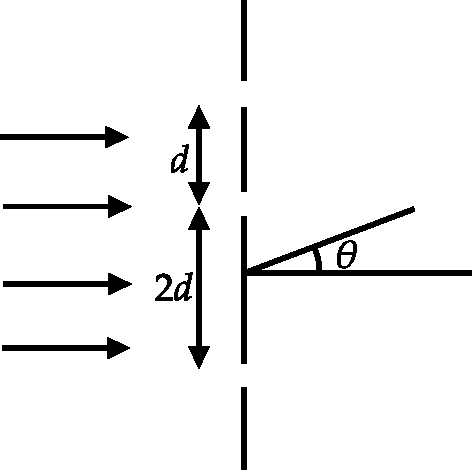
\includegraphics[height=3cm,width=5cm]{diagram-20211011(10)-crop}
	\end{figure}
\end{minipage}
\begin{tasks}(2)
	\task[\textbf{A.}] $2 \cos \delta+2 \cos 2 \delta$
	\task[\textbf{B.}]$3+\frac{1}{\delta^{2}} \sin ^{2} 3 \delta$
	\task[\textbf{C.}] $3+2 \cos \delta+2 \cos 2 \delta+2 \cos 3 \delta$
	\task[\textbf{D.}]$2+\frac{1}{\delta^{2}} \sin ^{2} 3 \delta$
\end{tasks}
\begin{minipage}{\textwidth}
	\item A monochromatic and linearly polarized light is used in a Young's double slit experiment.
	A linear polarizer, whose pass axis is at an angle $45^{\circ}$ to the polarization of the incident
	wave, is placed in front of one of the slits. If $I_{\max }$ and $I_{\min }$, respectively, denote the maximum and minimum intensities of the interference pattern on the screen, the visibility, defined as the ratio $\frac{I_{\max }-I_{\min }}{I_{\max }+I_{\min }}$, is
	\exyear{NET DEC 2018}
\end{minipage}
\begin{tasks}(2)
	\task[\textbf{A.}] $\frac{\sqrt{2}}{3}$
	\task[\textbf{B.}]$\frac{2}{3}$
	\task[\textbf{C.}]$\frac{2 \sqrt{2}}{3}$
	\task[\textbf{D.}]$\sqrt{\frac{2}{3}}$
\end{tasks}
\end{enumerate}
\colorlet{ocre1}{ocre!70!}
\colorlet{ocrel}{ocre!30!}
\setlength\arrayrulewidth{1pt}
\begin{table}[H]
	\centering
	\arrayrulecolor{ocre}
	
	\begin{tabular}{|p{1.5cm}|p{1.5cm}||p{1.5cm}|p{1.5cm}|}
		\hline
		\multicolumn{4}{|c|}{\textbf{Answer key}}\\\hline\hline
		\rowcolor{ocrel}Q.No.&Answer&Q.No.&Answer\\\hline
		1&\textbf{d}&2&\textbf{2}\\\hline
		3&\textbf{c}&4&\textbf{a}\\\hline
		5&\textbf{d}&6&\textbf{d}\\\hline
		7&\textbf{c}&8&\textbf{b}\\\hline
	\end{tabular}
\end{table}



\newpage 
\begin{abox}
	Practice set 2
	\end{abox}
\begin{enumerate}
	\begin{minipage}{\textwidth}
		\item Interference fringes are seen at an observation plane $z=0$, by the superposition of two plane waves $A_{1} \exp \left[i\left(\vec{k}_{1} \cdot \vec{r}-\omega t\right)\right]$ and $A_{2} \exp \left[i\left(\vec{k}_{2} \cdot \vec{r}-\omega t\right)\right]$, where $A_{1}$ and $A_{2}$ are real amplitudes. The condition for interference maximum is
		\exyear{GATE 2013}
	\end{minipage}
	\begin{tasks}(2)
		\task[\textbf{A.}] $\left(\vec{k}_{1}-\vec{k}_{2}\right) \cdot \vec{r}=(2 m+1) \pi$
		\task[\textbf{B.}]$\left(\vec{k}_{1}-\vec{k}_{2}\right) \cdot \vec{r}=2 m \pi$
		\task[\textbf{C.}] $\left(\vec{k}_{1}+\vec{k}_{2}\right) \cdot \vec{r}=(2 m+1) \pi$
		\task[\textbf{D.}] $\left(\vec{k}_{1}+\vec{k}_{2}\right) \cdot \vec{r}=2 m \pi$
	\end{tasks}
\begin{minipage}{\textwidth}
	\item In an interference pattern formed by two coherent sources, the maximum and minimum intensities are $9 I_{0}$ and $I_{0}$ respectively. The intensities of the individual wave are
	\exyear{GATE 2014}
\end{minipage}
\begin{tasks}(2)
	\task[\textbf{A.}] $3 I_{0}$ and $I_{0}$ 
	\task[\textbf{B.}]$4 I_{0}$ and $I_{0}$
	\task[\textbf{C.}]$5 I_{0}$ and $4 I_{0}$
	\task[\textbf{D.}]$9 I_{0}$ and $I_{0}$
\end{tasks}
\begin{minipage}{\textwidth}
	\item In a Young's double slit experiment using light, the apparatus has two slits of unequal widths. When only slit- 1 is open, the maximum observed intensity on the screen is $4 I_{0}$. When only slit-2 is open, the maximum observed intensity is $I_{0}$. When both the slits are open, an interference pattern appears on the screen. The ratio of the intensity of the principal maximum to that of the nearest minimum is
	\exyear{GATE 2015}
\end{minipage}

\end{enumerate}
\colorlet{ocre1}{ocre!70!}
\colorlet{ocrel}{ocre!30!}
\setlength\arrayrulewidth{1pt}
\begin{table}[H]
	\centering
	\arrayrulecolor{ocre}
	
	\begin{tabular}{|p{1.5cm}|p{1.5cm}||p{1.5cm}|p{1.5cm}|}
		\hline
		\multicolumn{4}{|c|}{\textbf{Answer key}}\\\hline\hline
		\rowcolor{ocrel}Q.No.&Answer&Q.No.&Answer\\\hline
		1&\textbf{b}&2&\textbf{b}\\\hline
		3&\textbf{9}&&\\\hline
	\end{tabular}
\end{table}












































